\documentclass{standalone}
\usepackage{tikz}
\usetikzlibrary{calc}
\usetikzlibrary{decorations.pathreplacing,calligraphy}
\usepackage{pgfplots}
\usetikzlibrary{intersections, pgfplots.fillbetween}
\usetikzlibrary{snakes}
\usepackage{xcolor}

\begin{document}


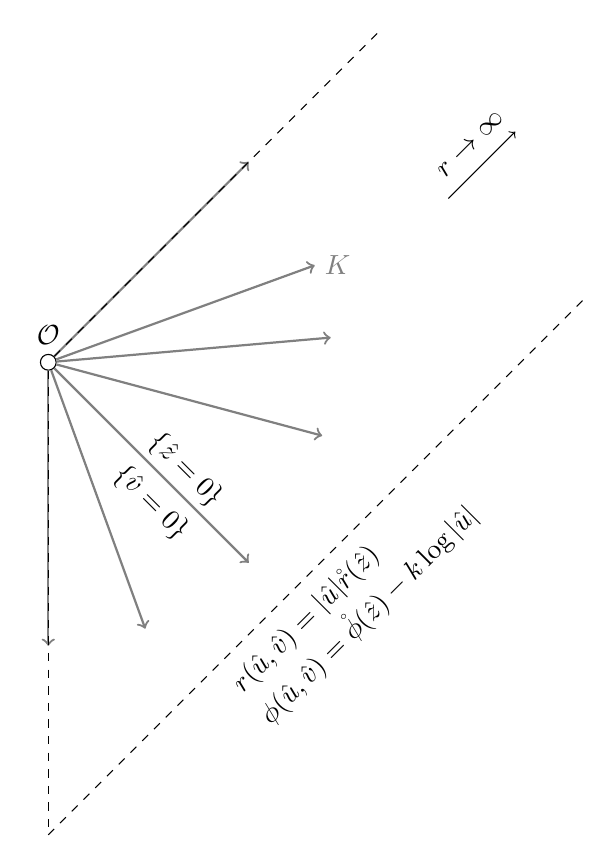
\begin{tikzpicture}[scale=1.2]
\node[circle, label= above:{$\mathcal{O}$}, draw, inner sep =0, minimum size = .2cm] (n1) at (0,0) {};

\coordinate (a1) at (-90:3);
\coordinate (a2) at (-70:3);
\coordinate (a3) at (-45:3);
\coordinate (a4) at (-15:3);
\coordinate (a5) at (5:3);
\coordinate (a6) at (20:3);
\coordinate (a7) at (45:3);

\draw[->, gray, thick] (n1) -- (a1);
\draw[->, gray, thick] (n1) -- (a2);
\draw[->, gray, thick] (n1) -- (a3);
\node[label = { [rotate=-45, yshift=-1.2mm, xshift=-.5mm]above:{$\{\hat{z}=0\} $ }     }] at (-45:2) {};


\draw[->, gray, thick] (n1) -- (a4);
\draw[->, gray, thick] (n1) -- (a5);
\draw[->, gray, thick] (n1) -- (a6);
\draw[->, gray, thick] (n1) -- (a7);

\node[label = right:{\textcolor{gray}{$K$}}] at ($(a6)+(-.1,0)$) {};

\draw[dashed] (n1) -- (0,-5);

\draw[dashed] (n1) -- (45:5);


\coordinate (a8) at (0,-5);

\draw[dashed] (a8) --+ (45:8);

\node[label = { [rotate=45, yshift=0mm, xshift=2mm]below:{$r(\hat{u},\hat{v}) = |\hat{u}|\mathring{r}(\hat{z})$ }     }] at ($(a8)+(45:3.5) $) {};
\node[label = { [rotate=45, yshift=5mm, xshift=8mm]below:{$ \phi(\hat{u},\hat{v}) = \mathring{\phi}(\hat{z}) - k \log|\hat{u}|$ }     }] at ($(a8)+(45:3.5)+(-45:.8) $) {};

\coordinate (f1) at ($(a6) + (45:1.5) + (-45:.5)$) ;
\coordinate (f2) at ($(a6) + (45:2.5) + (-45:.5)$) ;
\draw[->] (f1) -- (f2);
\node[label={[rotate=45]above:{$ r \rightarrow \infty $} } ] at ($(a6) + (45:2) + (-45:.5)$) {};

\node[label={[rotate=-45, yshift=.5mm, xshift=-3mm]below:{$ \{\hat{v}=0\} $} } ] at (-45:2) {};

\end{tikzpicture}

\end{document}